%%%%%%%%%%%%%%%%%%%%%%%%%%%%%
% Standard header for working papers
%
% WPHeader.tex
%
%%%%%%%%%%%%%%%%%%%%%%%%%%%%%

\documentclass[11pt]{article}

%%%%%%%%%%%%%%%%%%%%
%% Include general header where common packages are defined
%%%%%%%%%%%%%%%%%%%%



%%%%%%%%%%%%%%%%%%%%%%%%%%
%% TEMPLATES
%%%%%%%%%%%%%%%%%%%%%%%%%%


% Simple Tabular

%\begin{tabular}{ |c|c|c| } 
% \hline
% cell1 & cell2 & cell3 \\ 
% cell4 & cell5 & cell6 \\ 
% cell7 & cell8 & cell9 \\ 
% \hline
%\end{tabular}





%%%%%%%%%%%%%%%%%%%%%%%%%%
%% Packages
%%%%%%%%%%%%%%%%%%%%%%%%%%



% encoding 
\usepackage[utf8]{inputenc}
%\usepackage[T1]{fontenc}
\usepackage{ctex}

% general packages without options
\usepackage{amsmath,amssymb,amsthm,bbm}

% graphics
\usepackage{graphicx,transparent,eso-pic}

% text formatting
\usepackage[document]{ragged2e}
\usepackage{pagecolor,color}
%\usepackage{ulem}
\usepackage{soul}







%%%%%%%%%%%%%%%%%%%%%%%%%%
%% Maths environment
%%%%%%%%%%%%%%%%%%%%%%%%%%

%\newtheorem{theorem}{Theorem}[section]
%\newtheorem{lemma}[theorem]{Lemma}
%\newtheorem{proposition}[theorem]{Proposition}
%\newtheorem{corollary}[theorem]{Corollary}

%\newenvironment{proof}[1][Proof]{\begin{trivlist}
%\item[\hskip \labelsep {\bfseries #1}]}{\end{trivlist}}
%\newenvironment{definition}[1][Definition]{\begin{trivlist}
%\item[\hskip \labelsep {\bfseries #1}]}{\end{trivlist}}
%\newenvironment{example}[1][Example]{\begin{trivlist}
%\item[\hskip \labelsep {\bfseries #1}]}{\end{trivlist}}
%\newenvironment{remark}[1][Remark]{\begin{trivlist}
%\item[\hskip \labelsep {\bfseries #1}]}{\end{trivlist}}

%\newcommand{\qed}{\nobreak \ifvmode \relax \else
%      \ifdim\lastskip<1.5em \hskip-\lastskip
%      \hskip1.5em plus0em minus0.5em \fi \nobreak
%      \vrule height0.75em width0.5em depth0.25em\fi}



%%%%%%%%%%%%%%%%%%%%
%% Idem general commands
%%%%%%%%%%%%%%%%%%%%
%% Commands

\newcommand{\noun}[1]{\textsc{#1}}


%% Math

% Operators
\DeclareMathOperator{\Cov}{Cov}
\DeclareMathOperator{\Var}{Var}
\DeclareMathOperator{\E}{\mathbb{E}}
\DeclareMathOperator{\Proba}{\mathbb{P}}

\newcommand{\Covb}[2]{\ensuremath{\Cov\!\left[#1,#2\right]}}
\newcommand{\Eb}[1]{\ensuremath{\E\!\left[#1\right]}}
\newcommand{\Pb}[1]{\ensuremath{\Proba\!\left[#1\right]}}
\newcommand{\Varb}[1]{\ensuremath{\Var\!\left[#1\right]}}

% norm
\newcommand{\norm}[1]{\left\lVert #1 \right\rVert}



% argmin
\DeclareMathOperator*{\argmin}{\arg\!\min}


% amsthm environments
\newtheorem{definition}{Definition}
\newtheorem{proposition}{Proposition}
\newtheorem{assumption}{Assumption}

%% graphics

% renew graphics command for relative path providment only ?
%\renewcommand{\includegraphics[]{}}





\renewcommand{\abstractname}{Abstract}
\renewcommand\refname{References}
\renewcommand\figurename{Figure}

% comments and responses
\usepackage{xparse}
\usepackage{ifthen}
\DeclareDocumentCommand{\comment}{m o o o o}
{\ifthenelse{\draft=1}{
    \textcolor{red}{\textbf{C : }#1}
    \IfValueT{#2}{\textcolor{blue}{\textbf{A1 : }#2}}
    \IfValueT{#3}{\textcolor{ForestGreen}{\textbf{A2 : }#3}}
    \IfValueT{#4}{\textcolor{red!50!blue}{\textbf{A3 : }#4}}
    \IfValueT{#5}{\textcolor{Aquamarine}{\textbf{A4 : }#5}}
 }{}
}


% todo
\newcommand{\todo}[1]{
\ifthenelse{\draft=1}{\textcolor{red!50!blue}{\textbf{TODO : \textit{#1}}}}{}
}


%\usepackage[UTF8]{ctex}



% geometry
\usepackage[margin=2cm]{geometry}

% layout : use fancyhdr package
\usepackage{fancyhdr}
\pagestyle{fancy}

\makeatletter

\renewcommand{\headrulewidth}{0.4pt}
\renewcommand{\footrulewidth}{0.4pt}
\fancyhead[RO,RE]{\textit{Working Paper}}
\fancyhead[LO,LE]{G{\'e}ographie-Cit{\'e}s}
\fancyfoot[RO,RE] {\thepage}
\fancyfoot[LO,LE] {\noun{C. Losavio and J. Raimbault}}
\fancyfoot[CO,CE] {}

\makeatother


%%%%%%%%%%%%%%%%%%%%%
%% Begin doc
%%%%%%%%%%%%%%%%%%%%%

\begin{document}






%%%%%
% variable to include comments or not in the compilation ; set to 1 to include
\def \draft {1}
%\def \draft {0}



\title{Agent-based Modeling of Migrant Workers Residential Dynamics within a Mega-city Region: the Case of Pearl River Delta, China
}
\author{\noun{Cinzia Losavio} and \noun{Juste Raimbault}\\
UMR CNRS 8504 Géographie-cités
}
\date{}




\maketitle

\justify


\begin{abstract}
Over the last three decades, rural-to-urban migrant-workers have been a driving force for China's economy, raising attention on associated socio-economical issues. However, the importance of their economic diversity and social mobility has been poorly considered in the analysis of urban development strategy.
We use an agent-based model to simulate residential dynamics of migrants in Pearl River Delta (PRD) mega city region, taking into account the full range of migrants’ socio-economical status and their evolution. Mega-city regions have become a new scale of Chinese State regulation \comment[CL]{source ?}[(JR) oui oui][(CL)non non], and PRD represent the most prosperous and dynamic one in term of migration waves, standing as an ideal unit of analysis.
Our model unveils emergent patterns of dynamics, from micro behavior rules of discrete mobility choices. These choices are conditional to urban and economic environment, which evolution is controlled by meso-scale independent dynamics.
The two scales are coupled through the dependence of discrete choice utilities to generalized accessibility that combines patch-level urban and economic context with a feedback of the dynamics themselves. This multi-scale aspect is crucial to distinguish endogenous form exogenous effects in regional migration patterns.
We perform simulations to internally validate the model on synthetic data, by assessing statistical consistence and establishing phase diagrams across the parameter space.
The application to the case study allows first to test how variation in socio-economic status yield more complex trajectories, and secondly to identify how the Party-State persist in controlling internal migration flows in a more sophisticated and strategically redefined way.
Further work is directed towards a qualitative external validation of the model, by calibrating free parameters to reproduce meso-scale stylized facts, in order to guide interpretations of emergent outputs and potential policy applications.

\bigskip

\noindent\textbf{Keywords : } \textit{Mingong ; Residential Dynamics ; Agent-based Modeling ; Zhuijiang Delta Mega-city Region}
\end{abstract}




%%%%%%%%%%%%%%%%%%%%
\section{Introduction}


%%%%%%%%%%%%%%%%%%%%
\subsection{Context}

\paragraph{Mega-city Regions}

Mega-city regions (MCRs) are integrated sets of cities and their surrounding suburban hinterlands across which labour and capital can be reallocated at very low cost~\cite{florida2008rise}. The expression ``Mega-city Region'' was first coined by Gottmann~\cite{gottman1961megalopolis} using the term megalopolis, that he defines as “urban area of several tens of millions of people, including several cities and major urban centers, and extending continuously over several 100 km”. It represents the new economic unit that emerges as metropolitan regions not only grow upward and become denser but also grow outward and into one another. \comment{source ?} These spaces result of the networking of a group of metropolitan areas deployed around very large cities and it is characterized by the “symbiosis between urban and rural areas”.\comment{source ?}  Other characteristic are migration flows, density of connections, and regional migration patterns. 



\paragraph{Pearl River Delta}

Since the gradual decentralization of the state power which occurred in the beginning of  1990 Mega-city regions have become a new scale of Chinese State regulation, and in particular the pearl River Delta, represent the most prosperous and dynamic one in term of migration waves.\comment[CL]{check source} \comment[JR]{I found this paper \cite{xu2008governing} on governance of MCR in China, with PRD as case study ; maybe a good backup for the previous fact ? There is also this paper by Fulong Wu~\cite{wu2003post} studying how Shangai as an ``entrepreunarial city'' (to be distinguished from entrepreunarial activities in the city, in the sense that the first corresponds to structural spatial actions to raise competitiveness) is an initiative and strategy of the ``Post-Socialist State''.}
That’s why we choose PRD as our unit of study. Since the Open Door Policy was implemented in 1978 the PRD launched a process of rapid economic and social transformation, becoming a global manufacturing region attracting an increasing number of migrant-workers from all over China. In fact, PRD was designed as an open economic zone in 1984, and was granted many ‘one step ahead’ policies to attract foreign capital, becoming the most important exporter center since economic reform. That results in an astonishing rise of population in the area. That today count more than 50 million people.\comment{source ?} If during the first year of the opening-up reforms the barycenter of the region was Guangzhou - the provincial capital, over the last decade PRD has become increasing polycentric.
Taking PRD as the unit of our model we try to reproduce migrants residential patterns taking into account the full range of migrants’ socio-economical status and their evolution. 



\paragraph{Migrant Workers in PRD}


Even though migrants workers are generally considered and treated as a uniform category, previous research~\cite{losavio2016analyser}, based on qualitative interviews and sociological observation, showed how considering their economical, cultural and human capital migrants workers are a very diversified social category. Especially 3 dimension are fundamental to understand migrant workers:
\begin{itemize}
\item Professional Dimension : industry, construction, private sector, services (will change not only their economical situation but which influence  migrants’ trajectory and the staying duration in the city and their residential choice.
\item Residential Dimension : We could recognize two subcategories, with different socio-economic situations: (i) Temporary - migrants working in the construction sector, who are really mobile, changing city or province according to the labour demand;  seasonal migrants workers, most of the time are peasants working as farmer and cultivating their land who come to the urban area to sell their product at the city price but without paying the running costs temporary migrants’ trajectory are more difficult to detect since they move in a discretional way ; (ii) Permanent :  Who are living in the city for more than 6 months and are renting a room or apartment depending on their: Economic situation (revenues), Social network, Proximity to the work place
\item Generational Dimension. \textit{this dimension is not taken into account in the model for now, as simulated dynamics correspond to rather short time scales, between 10 and 20 years.}
\end{itemize}


All these sub-categories have different mobility patterns, that we try to simulate in our model.

Considering this diversity and translating it in qualitative stylized facts that correspond to precise patterns of synthetic data, this model aims at establishing a new perspective for understanding China’s urban and regional mobility employing a more qualitative approach, specifying the mechanisms through which Party-State shape the parameters of migrants’ choices. \comment[CL]{The points-based hukou system represents one of these mechanisms. It would be great to add it into the model.}[(JR) Yes indeed, I'm looking into that.]





%%%%%%%%%%%%%%%%%%%%
\subsection{Modeling Migrations}

% agent-based model in Urban Studies : http://journals.sagepub.com/doi/pdf/10.1177/0042098009346326
% http://en.cnki.com.cn/Article_en/CJFDTotal-CSFY200909013.htm
% http://www.tandfonline.com/doi/full/10.1111/j.1467-8306.2007.00559.x?scroll=top&needAccess=true : CA model of Desakota (rurban expansion)

\paragraph{Modeling Rural-urban migrations}

\cite{todaro1969model} classical equilibrium model


\paragraph{Modeling Rural-urban migrations in China}

Existing works in rural-urban migration modeling in China are mainly econometric studies, relying on census or on survey data. \cite{zhang2013measuring} estimate discrete choice models to study the trade-off between migration distance and earning difference. \cite{fan2005modeling} shows that gravity-based models can explain well inter-provincial migratory patterns, implying an underlying strong dominant aggregation processes. The positive association between wage gap and migration rates was obtained from time-series analysis in~\cite{zhang2003rural}. An empirical study of intra-urban migrants residential dynamics is done by~\cite{wu2006migrant}.



\comment[JR]{\cite{2017arXiv170600682Y} : big data analysis of migrants spatio-temporal behavior}


\paragraph{Towards an agent-based modeling approach}

To the best of our knowledge, there was no attempt in the literature before to focus on China's migration issues from an agent-based perspective. The case of Mexico was tackled by~\cite{de2007netlogo}, but in the particular case of a border-town, and underlying processes are furthermore fundamentally different.

\cite{xie2007simulating} : agent-based model to simulate the emergence of Urban Villages. \cite{silveira2006agent} : Ising model of rural-urban migration. \cite{fernandez2005characterizing} : study of population characteristics to establish the relevance of a future ABM. \comment{I think later we should comment a bit more the litterature you cite here!}[yes of course]

The idea of applying complexity paradigms to rural-urban migration is far from new, as~\cite{mabogunje1970systems} already theorized it in the frame of General System Theory, that for some is viewed as a precursor of complexity theories. \comment{Was there a particular study? If is we can be more precise at least on the country where this kind of pattern has been studied}[it is a fully theoretical paper (although the empirical inspirations seem to be from Nigeria). the citation was more to justify our theoretical and methodological background, we'll have to think if it is really appropriate]

Following a logic of \emph{Pattern-oriented modeling}~\cite{grimm2005pattern}, combined with recent advances in multi-modeling~\cite{cottineau2016back}, one can use agent-based models as powerful tools to test qualitative hypothesis, with a reasonable need for empirical data through toy-models or hybrid models.



%%%%%%%%%%%%%%%%%%%%
\section{Model}

\subsection{Rationale}

We choose to focus on particular processes and stylized facts to include in the agent-based models \comment{modif.}, in order to test some hypothesis formulated after qualitative research done in~\cite{losavio2016analyser}. More precisely, a recent shift in socio-economic structure of migrating population was observed, including a rise of middle-income migrants and a relativisation of the role of \emph{Hukou} in migration dynamics. The core of the model is thus centered on the exploration of the impact of a varying population economic structure for migrants on system dynamics, and the influence of government migration policies.

\paragraph{Scale} As shown by~\cite{chan2012migration}, since last three decades (since the Deng Xiaoping economic reforms) migration dynamics features reveal a high asymmetry from central regions to coastal economically dynamic province. At a macroscopic scale, explanatory variables are relatively well understood and gravity-based geographical models have a reasonable explanatory power~\cite{fan2005modeling}. However, at a regional scale, migration dynamics are also highly present and present more complex patterns. The scale of the model is therefore a regional scale, in the spirit of a \emph{Mega-city Region} \cite{hall2006polycentric}, in which urban dynamics are highly complex. A relevant case study to apply the model will be the Pearl River Delta Region in Guangdong.

\paragraph{Ontology} At a mesoscopic scale, i.e. for cities within the MCR, growth can be reasonably assumed as independent from migrants movements : they follow larger economic urban processes. Conditionally to such population and economic context, migration dynamics occur at the microscopic scale. We postulate a simple utility-maximization process.


%%%%%%%%%%%%%%%
\begin{figure}
\centering
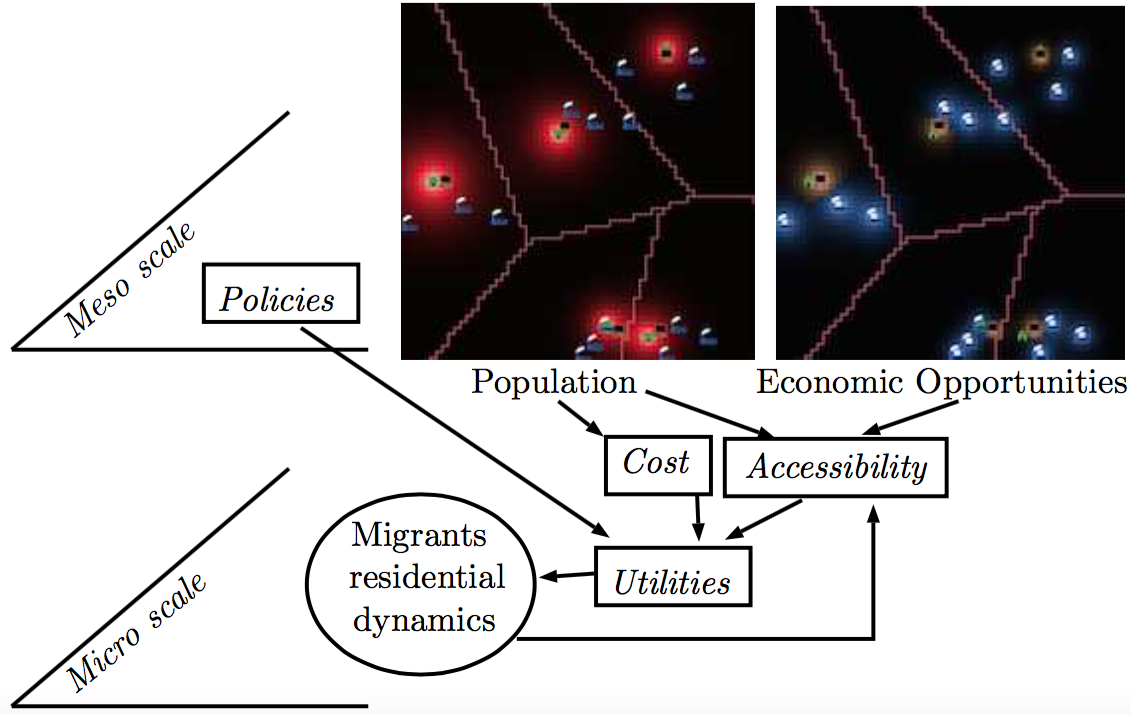
\includegraphics[width=\textwidth]{figures/model}
\caption{Multi-scale schema of processes included in the model}
\label{fig:model}
\end{figure}
%%%%%%%%%%%%%%%


\subsection{Model Description}

\paragraph{Setup}

The world \comment{Why do you talk about the “world” ? Do you mean the world of our model?}[yes it is a term for the space of the model] consists in a lattice of $1 \leq i \leq N$ cells, characterized by their population $P_i(t)$ and an economic structure $E_i^{(c)}(t)$ which consists in abstract variables representing potential number of jobs stratified by socio-economic classes $c$. The associated effective number of workers is denoted by $W_i^{(c)}(t)$. For the sake of simplicity, we assume a discrete number of classes. At initial time, the variables are initialized either following a synthetic data generation process (see below), or from real geographical data (abstracted and simplified to fit our context). Cells are grouped into $1\leq k\leq K$ administrative cities that corresponding to the various centers of the MCR, on which aggregated population $\tilde{P}_k(t)$ and corresponding economic variables ($\tilde{E}_k^{c}(t)$) can be computed.

\newpage

\paragraph{Agents}

An agent is a household of migrants, whose residence and job are located in cells (that can be different). Socio-economic structure of the population is captured by the distribution of wealth $g(w)$, which are then stratified into categories. At a given time, the utility difference between not moving and moving to cell $j$ from cell $i$, for a category $c$ is given by

\[
\Delta U_{i,j}^{(c)}(t) = \frac{Z_j^{(c)}- Z_i^{(c)}}{Z_0} + \gamma \cdot \frac{C_i^{(c)}- C_j^{(c)}}{C_0} - u_i^{(c)} - h_j^{(c)}
\]

where $Z_i^{(c)}$ is generalized accessibility given by $Z_i^{(c)} = P_i \cdot \sum_k \left[E_k^{(c)}-W_k^{(c)}\right]\cdot \exp{\left(\frac{-d_{ij}}{d_0}\right)}$, with $d_{ij}$ effective travel distance \footnote{as the model does not focus on the role of transportation, we take euclidian distance, and $d_0$ captures typical commuting distance in both public transportation or car. A more complex model could include an explicit transportation network and modal choice depending on socio-economic category.} and $d_0$ commuting characteristic distance ; the parameter $\gamma$ is the ratio giving the relative importance of life cost compared to accessibility in the migration decisions ; $C_i^{(c)}$ is the cost of life which is a function of cell and city variables, that will be taken as $C_i^{(c)} \propto P_i^{\alpha_0}\cdot  \tilde{P}_i^{\alpha_1}\cdot$ ; $u_i^{(c)}$ a baseline aversion to move and $h_j^{(c)}$ an exogenous variable corresponding to regulation policies ; $Z_0$ and $C_0$ dimensioning parameters.

\paragraph{Temporal Evolution}

At each time step, the system evolves sequentially according to the following rules :

\begin{enumerate}
\item Cities mesoscopic variables $\tilde{P}_k(t)$ and $\tilde{E}_k^{c}(t)$ are deterministically updated. Population follows the very simple assumption of the expectancy of a Gibrat's law, i.e. $\tilde{P}_k(t)= g_k \cdot \tilde{P}_k(t-1)$. Economy follows a scaling law of population: $\tilde{E}_k^{(c)}(t) = E_k^{(c,0)}\cdot \left(\frac{\tilde{P}_k(t)}{P_0}\right)^{\gamma_k^{(c)}}$.

\item Patches variables are updated conditionally to the new aggregated values. For population, we adapt the aggregation-diffusion process detailed in~\cite{raimbault2016calibration}: a density ceil is introduced and diffusion is replaced by spatial noise. More precisely, let $\Delta \tilde{P}_k(t) = \tilde{P}_k(t) - \tilde{P}_k(t-1)$. \comment{less clear for me}[this part is unfinished indeed]

\item A number $M$ of new migrants, enters the region. They lean on social network %(关系,guanxi) \comment{(CL) ADD EXPLICATIVE NOTE}
to first settle in the city and agglomerate following a preferential attachment by place of origin.
\item Migration occur following a discrete choice dynamics : the probability to move to cell $j$ is given by

\[
\Pb{i\rightarrow j | c} = \frac{\exp{\left(\beta\cdot U_j^{(c)}\right)}}{\sum_k \exp{\left(\beta\cdot U_k^{(c)}\right)}+\exp{\left(U_{stay,i}^{(c)}\right)}}
\]

what simplifies into a reduced form, with $\beta' = \frac{\beta}{Z_0}$, $\gamma' = \frac{\gamma}{Z_0C_0}$ and $\tilde{u},\tilde{h}$ accordingly rescaled variables, using the above utility expression :

\[
\Pb{i\rightarrow j | c} = \frac{\exp{\left(\beta'\cdot \left[\Delta Z_{i,j}^{(c)} - \gamma' \cdot \Delta C_{i,j}^{(c)} - \tilde{u}_i^{(c)} - \tilde{h}_j^{(c)} \right] \right)}}{1 + \sum_k {\exp{\left(\beta'\cdot \left[\Delta Z_{i,k}^{(c)} - \gamma' \cdot \Delta C_{i,k}^{(c)} - \tilde{u}_i^{(c)} - \tilde{h}_k^{(c)} \right] \right)}}}
\]

Residential movement is drawn randomly according to these probabilities, and jobs are chosen around new residence following an exponentially decreasing probability.

\item Migrants update their wealth and eventually economic category, according to an abstract ``quality of place'' that we associate to per-capita GDP which follows a scaling law of population

%population / max-population * [city-population] of owning-city / economic-p0
% note : tunable function : test its role !

\[
w = w\cdot \left( 1 + g_{w} \frac{P_i}{\max P_j} \cdot \frac{\tilde{P}_k}{\max \tilde{P}_l} \right)
\]

\end{enumerate}


\paragraph{Indicators}

The outcome of the model has many dimensions, and is measured through the following indicators :

\begin{itemize}
\item Total migrants wealth gain
\item Total migrants social mobility
\item Cumulated utility difference in migrations: when someone migrates, it corresponds to a given utility gain $\Delta U$ : this indicator is $\sum \Delta U^{(c)}$ on all realized migrations for each category.
\item Inequalities are captured by the final ratio between socio-economic categories
\end{itemize}


\paragraph{Synthetic Data Generation}

A synthetic mega-city region is generated following simple stylized facts for systems of cities. A polycentric structure, each center having an exponential density decay, is created with random coordinates for centers. Population of centers follow a rank-size law of slope 1.2.


\paragraph{Parameters}

We summarise main parameters in table~\ref{tab:parameters}.

\begin{table}
\caption{Summary of main parameters\label{tab:parameters}}
\bigskip
\centering
\begin{tabular}{ |c|c|c|c| } 
\hline
Parameter & Name & Values & Process  \\\hline
$\gamma$ & Cost/Accessibility ratio & $\log\gamma \in \left[5;8\right]$ & Mobility \\ 
$u_0$ & Move aversion & $u_0\in\left[0;5\right]$ & Risk aversion \\ 
$\beta$ & Discrete Choices & $\beta\in \left]0;+\infty\right[$ & Determinism \\ 
$g_w$ & Income Growth & $g_w \in \left[0;1\right]$ & Wealth Increase  \\
$d_0$ & Accessibility Decay & $d_0\in \left]0;+\infty\right[$ & Accessibility \\ 
$\sigma$ & Wealth dispersion & $\sigma\in \left[0.1;1.0\right]$ & Economic Inequalities \\ 
\hline
\end{tabular}
\end{table}



%%%%%%%%%%%%%%%%%%%%
\section{Results}
%%%%%%%%%%%%%%%%%%%%




\todo{
Next steps :
\begin{itemize}
\item Full exploration on synthetic data : model behavior
\item Stylization and scenarization of real PRD configuration, model behavior on real and hybrid configurations
\item Targeted experience plans (e.g. : role of economic diversity, influence of state regulation)
\item Iterative further construction/multi-modeling (e.g. generations)
\end{itemize}
Expected Results :
\begin{itemize}
\item Impact of processes linked to migrants diversities on emergent dynamics
\item Explore or unveil state strategies (through regulations or companies control \comment{why companies control ?}[I had in mind a possible action on company locations ?])
\end{itemize}
}



%%%%%%%%%%%%%%%%%%%%
\subsection{Model Validation and Baseline Exploration}

\paragraph{Internal validation} 

statistical consistence : cf Fig.~\ref{fig:statistical-valid} ; system trajectories ; path-dependency.

%%%%%%%%%%%%%%%%
\begin{figure}
\centering
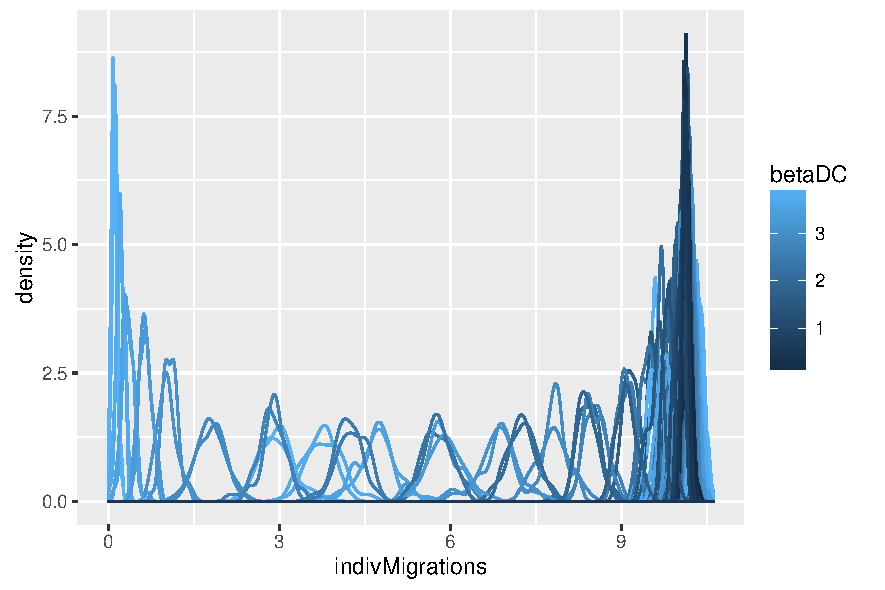
\includegraphics[width=0.48\textwidth]{figures/baseline_hist_indivMigrations_colorbetaDC}
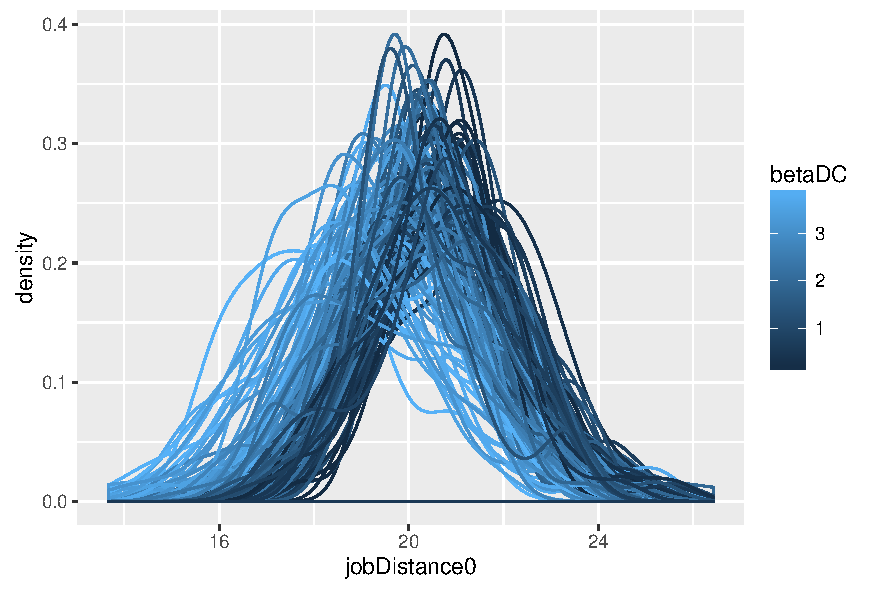
\includegraphics[width=0.48\textwidth]{figures/baseline_hist_jobDistance0_colorbetaDC}
\caption{Statistical distributions of number of individual migrations and wealth gain over 50 runs, for some example parameter points}
\label{fig:statistical-valid}
\end{figure}
%%%%%%%%%%%%%%%%




\paragraph{External validation : baseline behavior}

We first establish the behavior of the model on the simplest baseline situation, to which will be compared more complex parameter configurations. The baseline assumes no city growth ($g_k=1$), no external migration ($M=0$), no income growth ($g_{w}$), $u_i$ is fixed at a constant value $U_0$ and we have only one economic category. Fig.~\ref{fig:baseline-indics} show indicator values across the parameter space.

We extract the following stylized facts from model behavior :
\begin{itemize}
\item As expected, we observe a phase transition in number of migrations for increasing $\beta$ ; the transition points increases when $u_0$ decreases, until the model follows a change in qualitative behavior (bifurcation ?) : increasing $\beta$ first produces a peak in migrations before they fall down again. The increase above 1 migration per migrant and per time step is possible by the disappearance of some of them due to a saturation of jobs. \textit{When migrants have a high propensity to move, the spatial repartition of jobs becomes suboptimal in intermediate regimes of stochasticity, corresponding to a regime where congestion dominates.} \comment{fact to be compared with the real config, maybe it is due to the spatial structure ; try to trickle also job number parameters, meta-parameter of synthetic system shape.}
\item The previous observation is consistent with the behavior of the average distance to job (this plot is quite noisy as it depends on spatial configuration, stabilizing it would thus need supplementary repetitions, as the exploration for sensitivity of meta-parameters) : it always decreases with $\beta$, but individual move repulsion changes the shape. Low values give a linear decrease of job distance with $\beta$, whereas high values produce a saturating curve that becomes constant. \textit{The congestion regime corresponds to a linear decrease of job distance with randomness, meaning that social determinism creates spatial inequalities.}
\item Not sensitive to $\gamma$ : the sensitivity to ratio cost/accessibility is very low \comment{(CL) to job or to city ?}[(JR) jobs, we work with generalized accessibility, see below], what may be due to the dependence of dynamics to outliers of utility distributions : its central shape changes a lot with it but not extreme values. \textit{Changing the relative importance of accessibility does not affect much the aggregated dynamics : an increased gain in mobility produced by policies for examples will have no effect on migrations patterns.} \todo{plot the patch distrib of utilities ? (in netlogo) $\rightarrow$ some examples }
\item Temporal Dynamics : Fig.~\ref{fig:migr-diff}. The dependence of dynamics to parameter is much richer ; we observe a transition from a maximum, to a min, and then a max again. In configurations averse to move, time has a positive feedback on migrations ; intermediate situations show a negative feedback (progressive saturation in time) ; to switch again to a positive feedback in most mobile situations. \textit{Configurations with an intermediate value of move aversion (in which real configurations fall) yield a negative feedback effect to time, witnessing a progressive saturation. In a ``U-shape'' manner, very mobile or very fixed configurations yield positive feedback of time.} \comment{(JR) note : this directs to the exploration of not constant but proba distrib for $u_i$ ; or function of something ? no it is an externality !}
\end{itemize}



%%%%%%%%%%%%%%%%
\begin{figure}
\centering
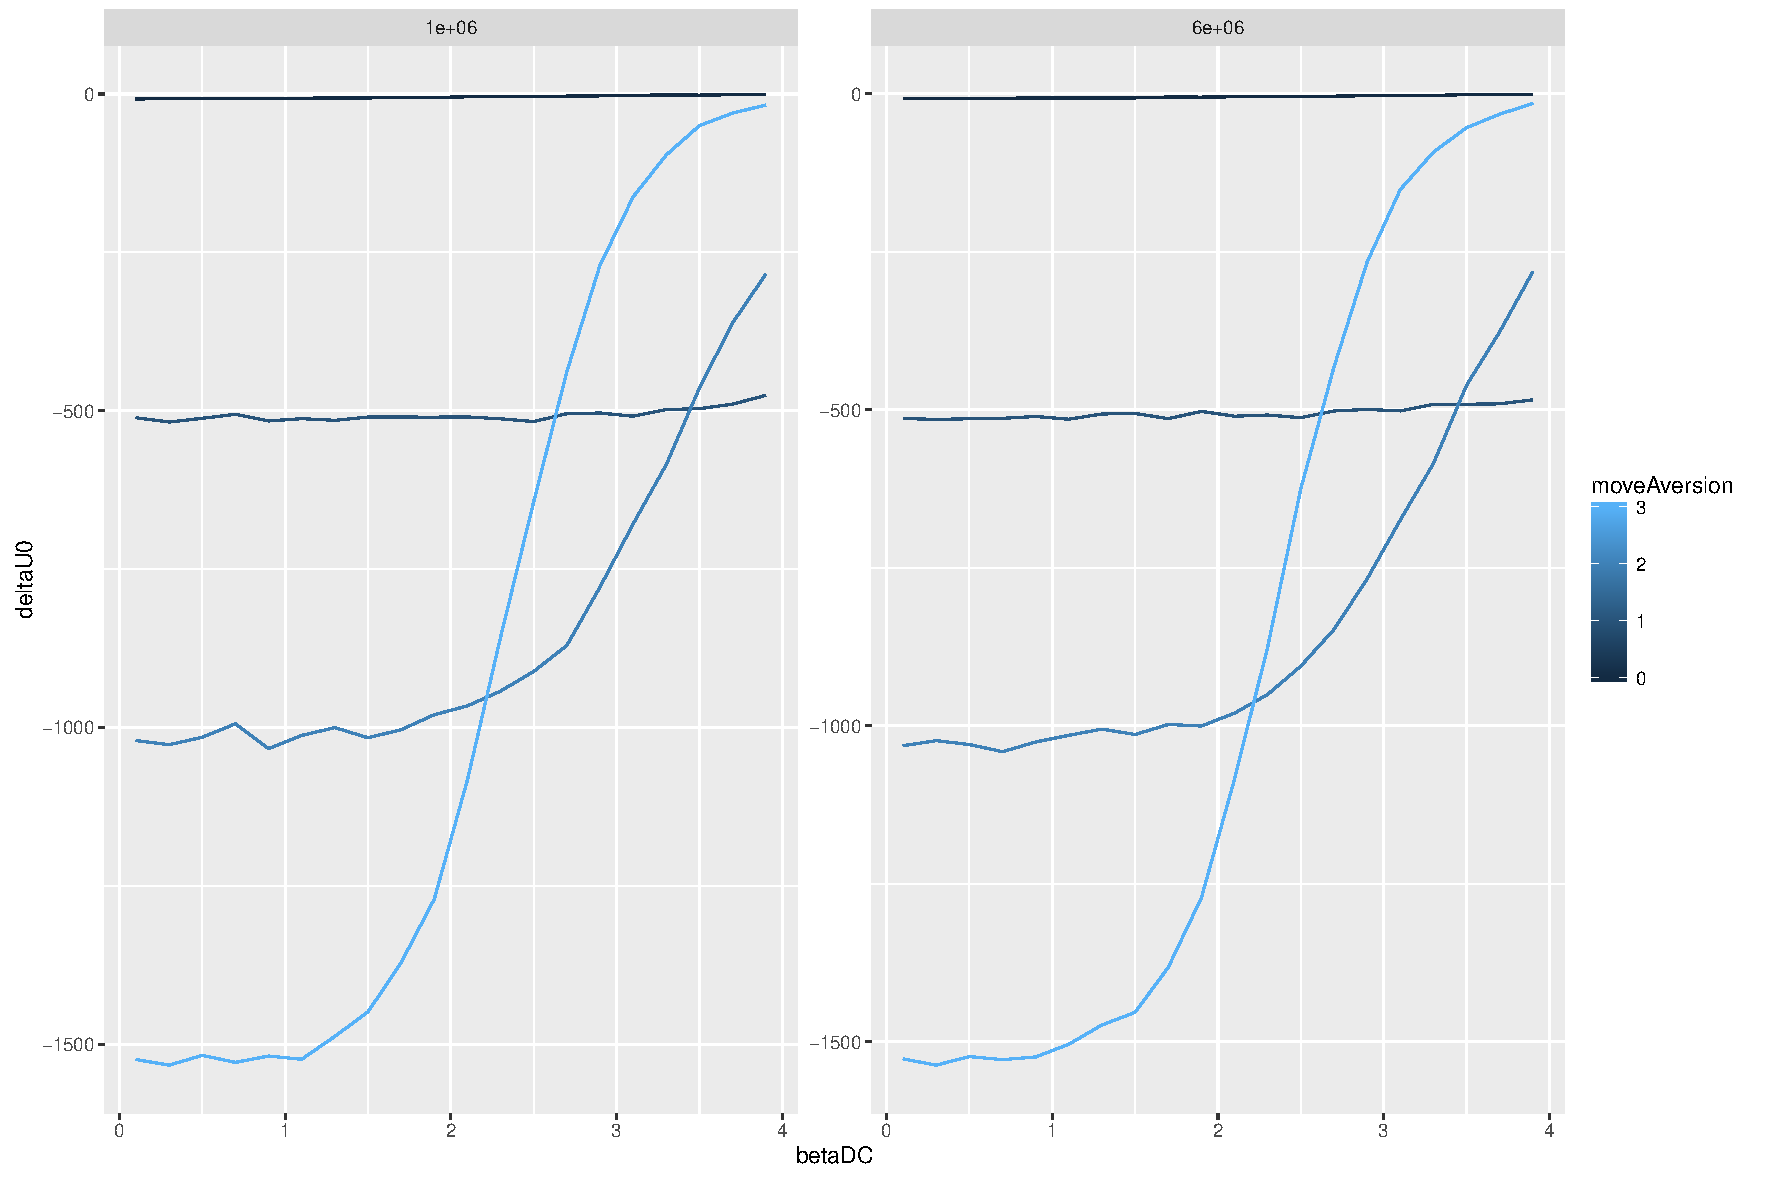
\includegraphics[width=0.48\textwidth]{figures/baseline_indicdeltaU0}
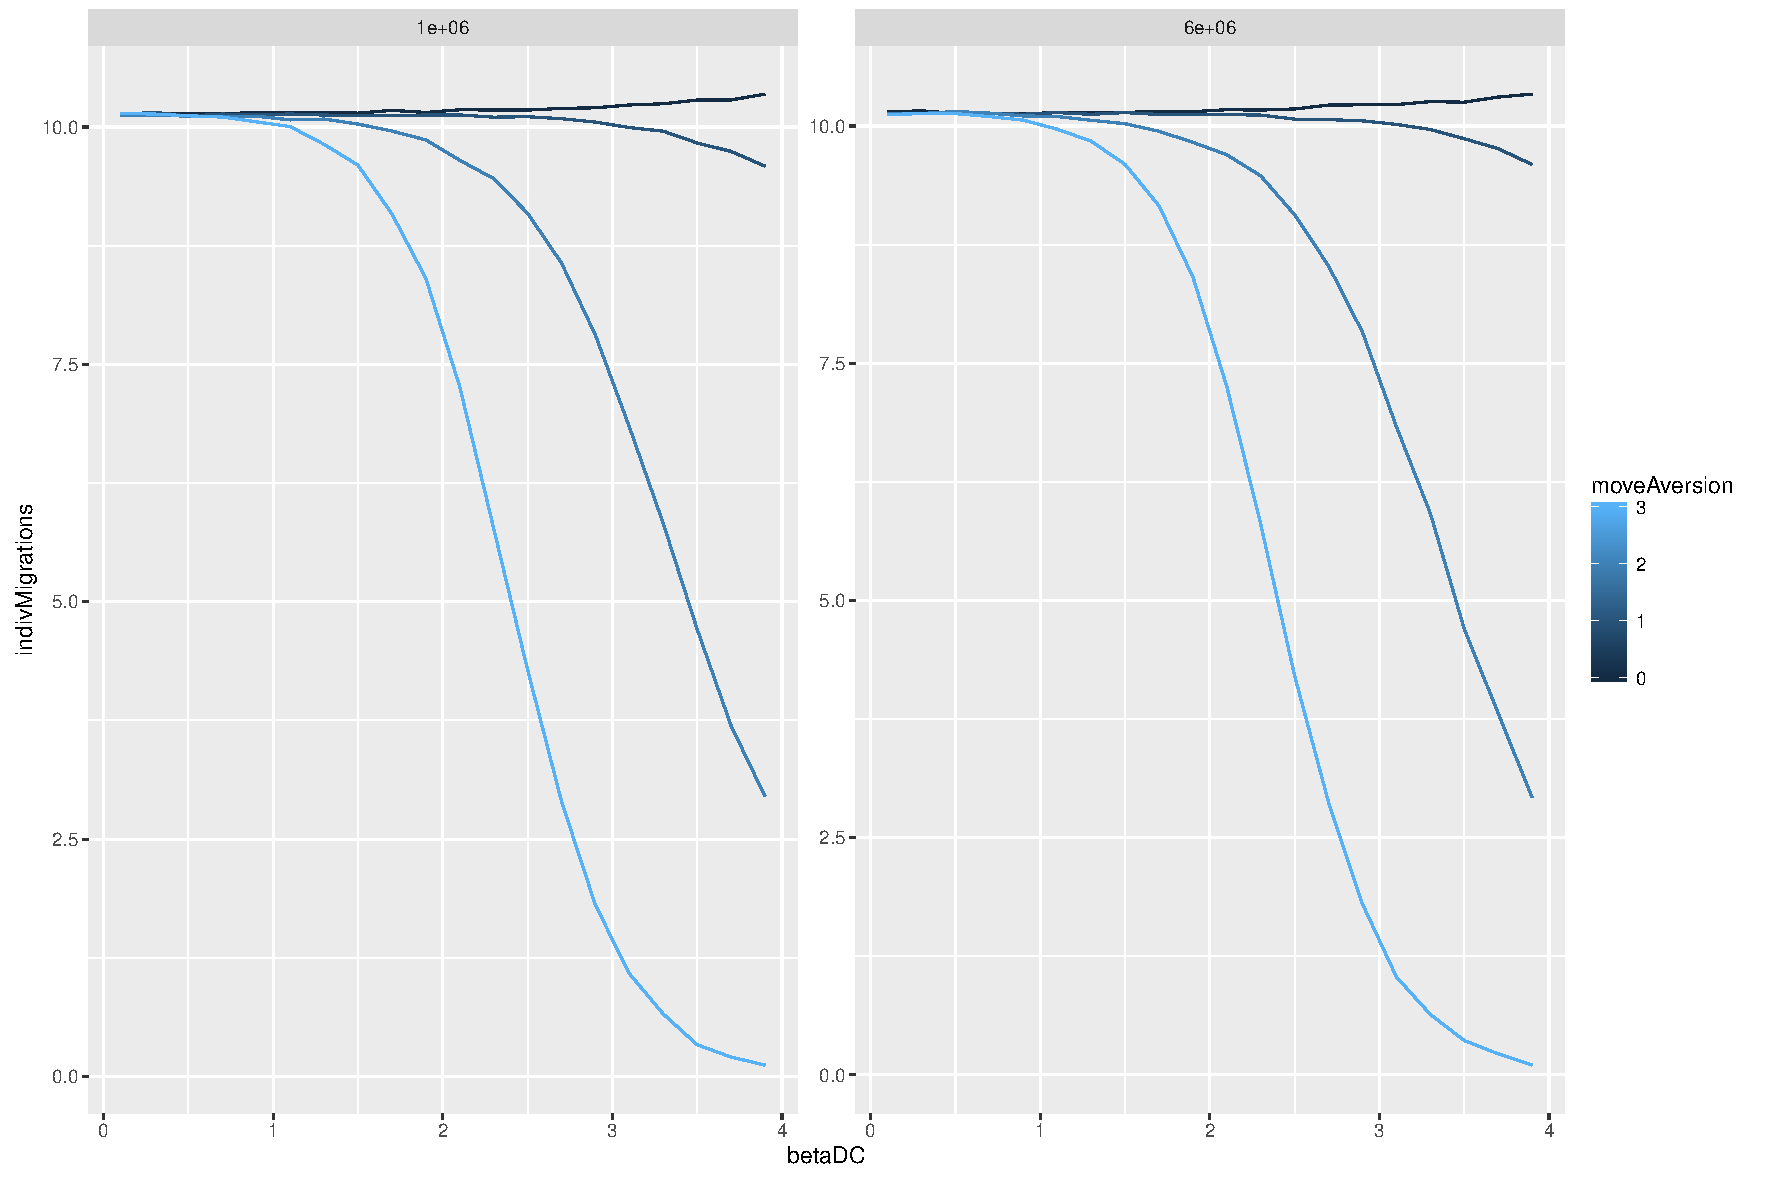
\includegraphics[width=0.48\textwidth]{figures/baseline_indicindivMigrations}\\
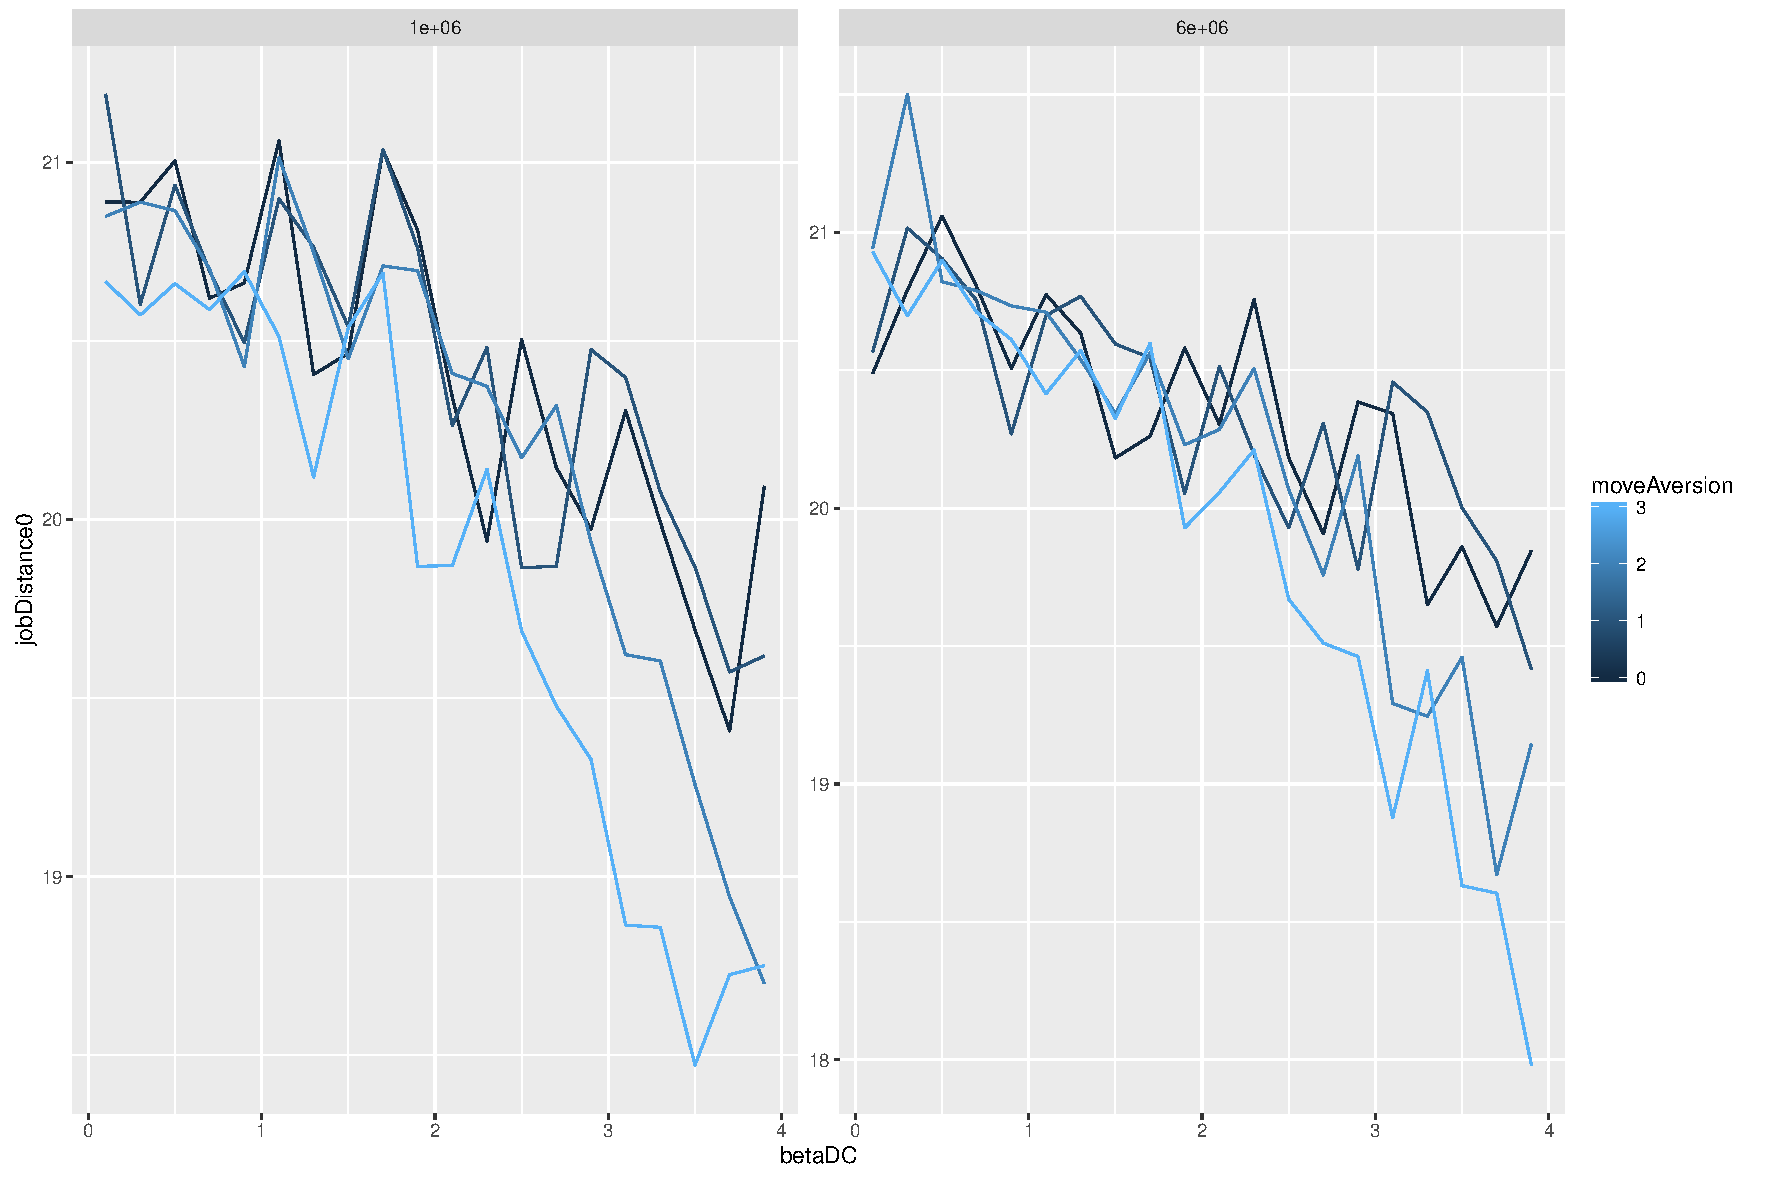
\includegraphics[width=0.48\textwidth]{figures/baseline_indicjobDistance0}
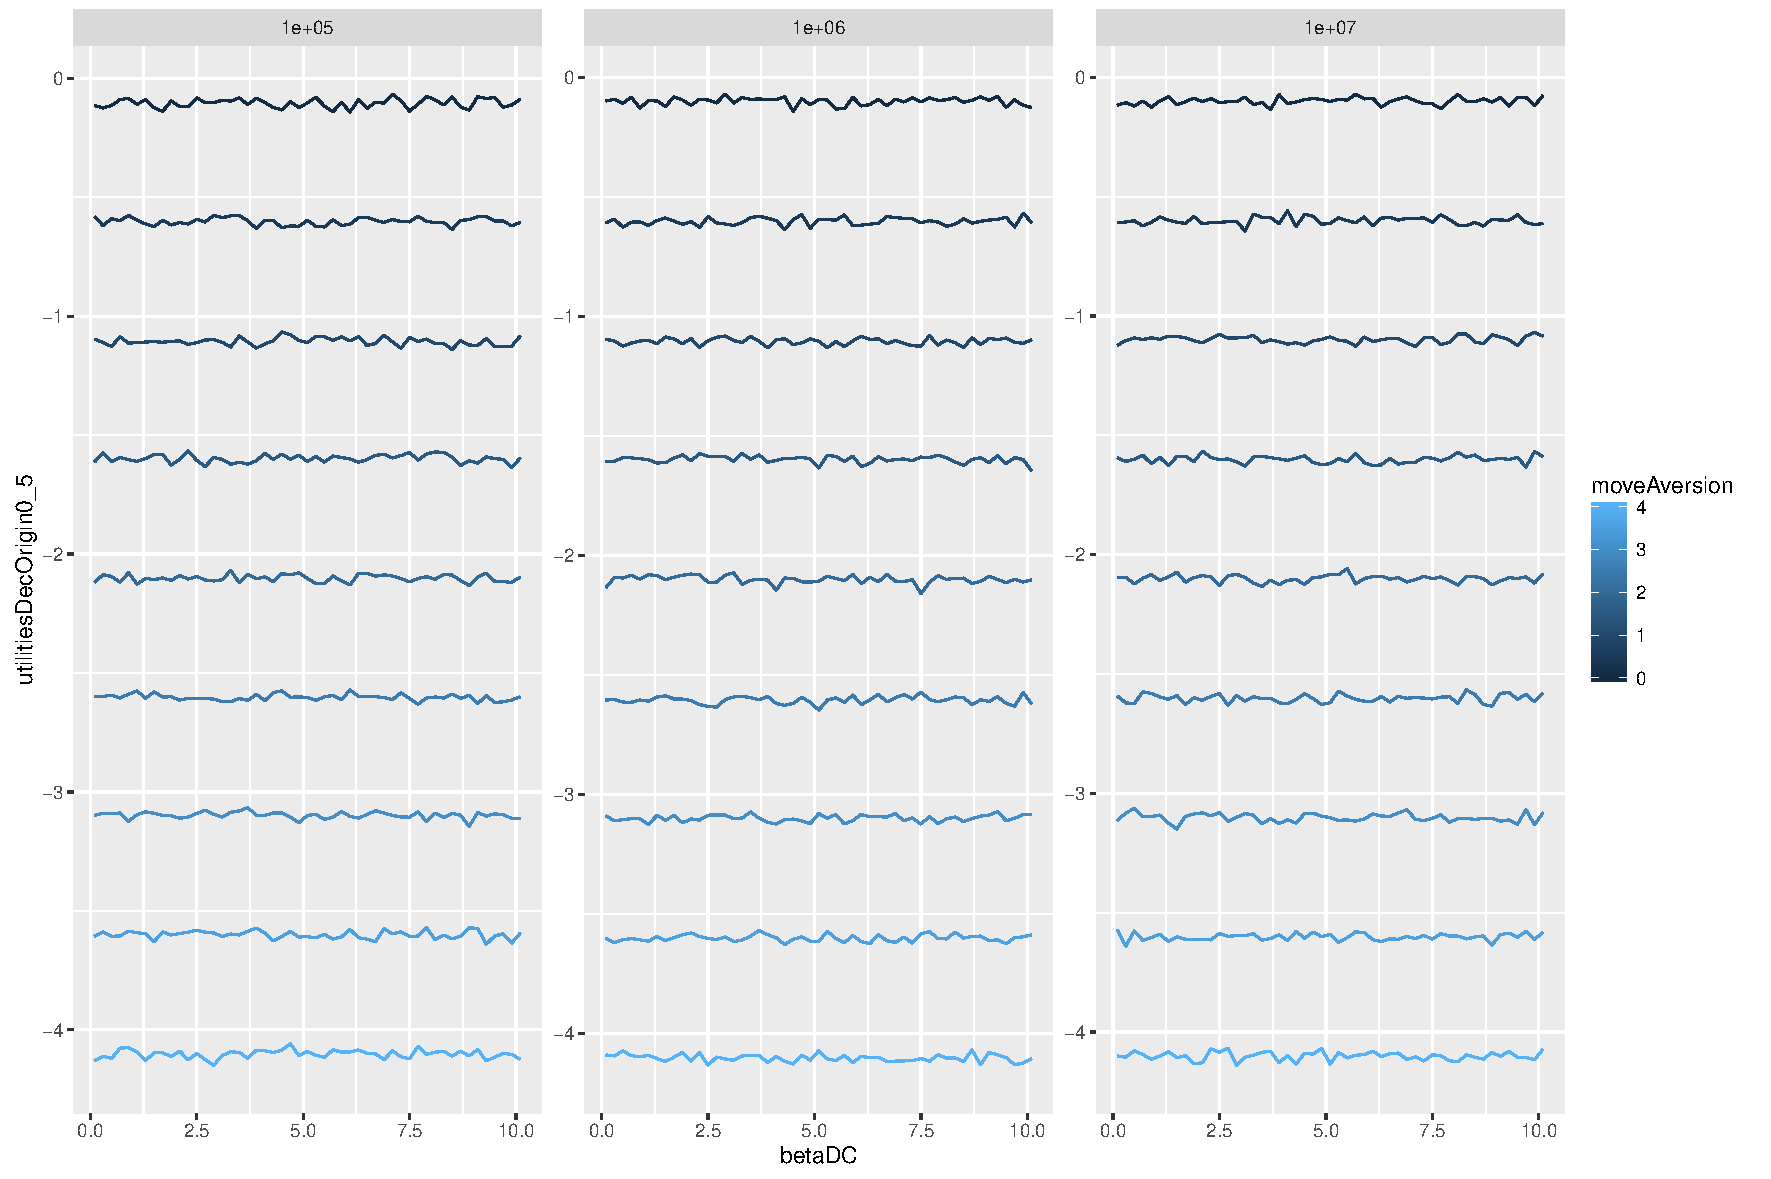
\includegraphics[width=0.48\textwidth]{figures/baseline_indicutilitiesDecOrigin0_5}
\caption{Model behavior, averaged over 50 runs, for a baseline configuration.}
\label{fig:baseline-indics}
\end{figure}
%%%%%%%%%%%%%%%%


%%%%%%%%%%%%%%%%
\begin{figure}
\centering
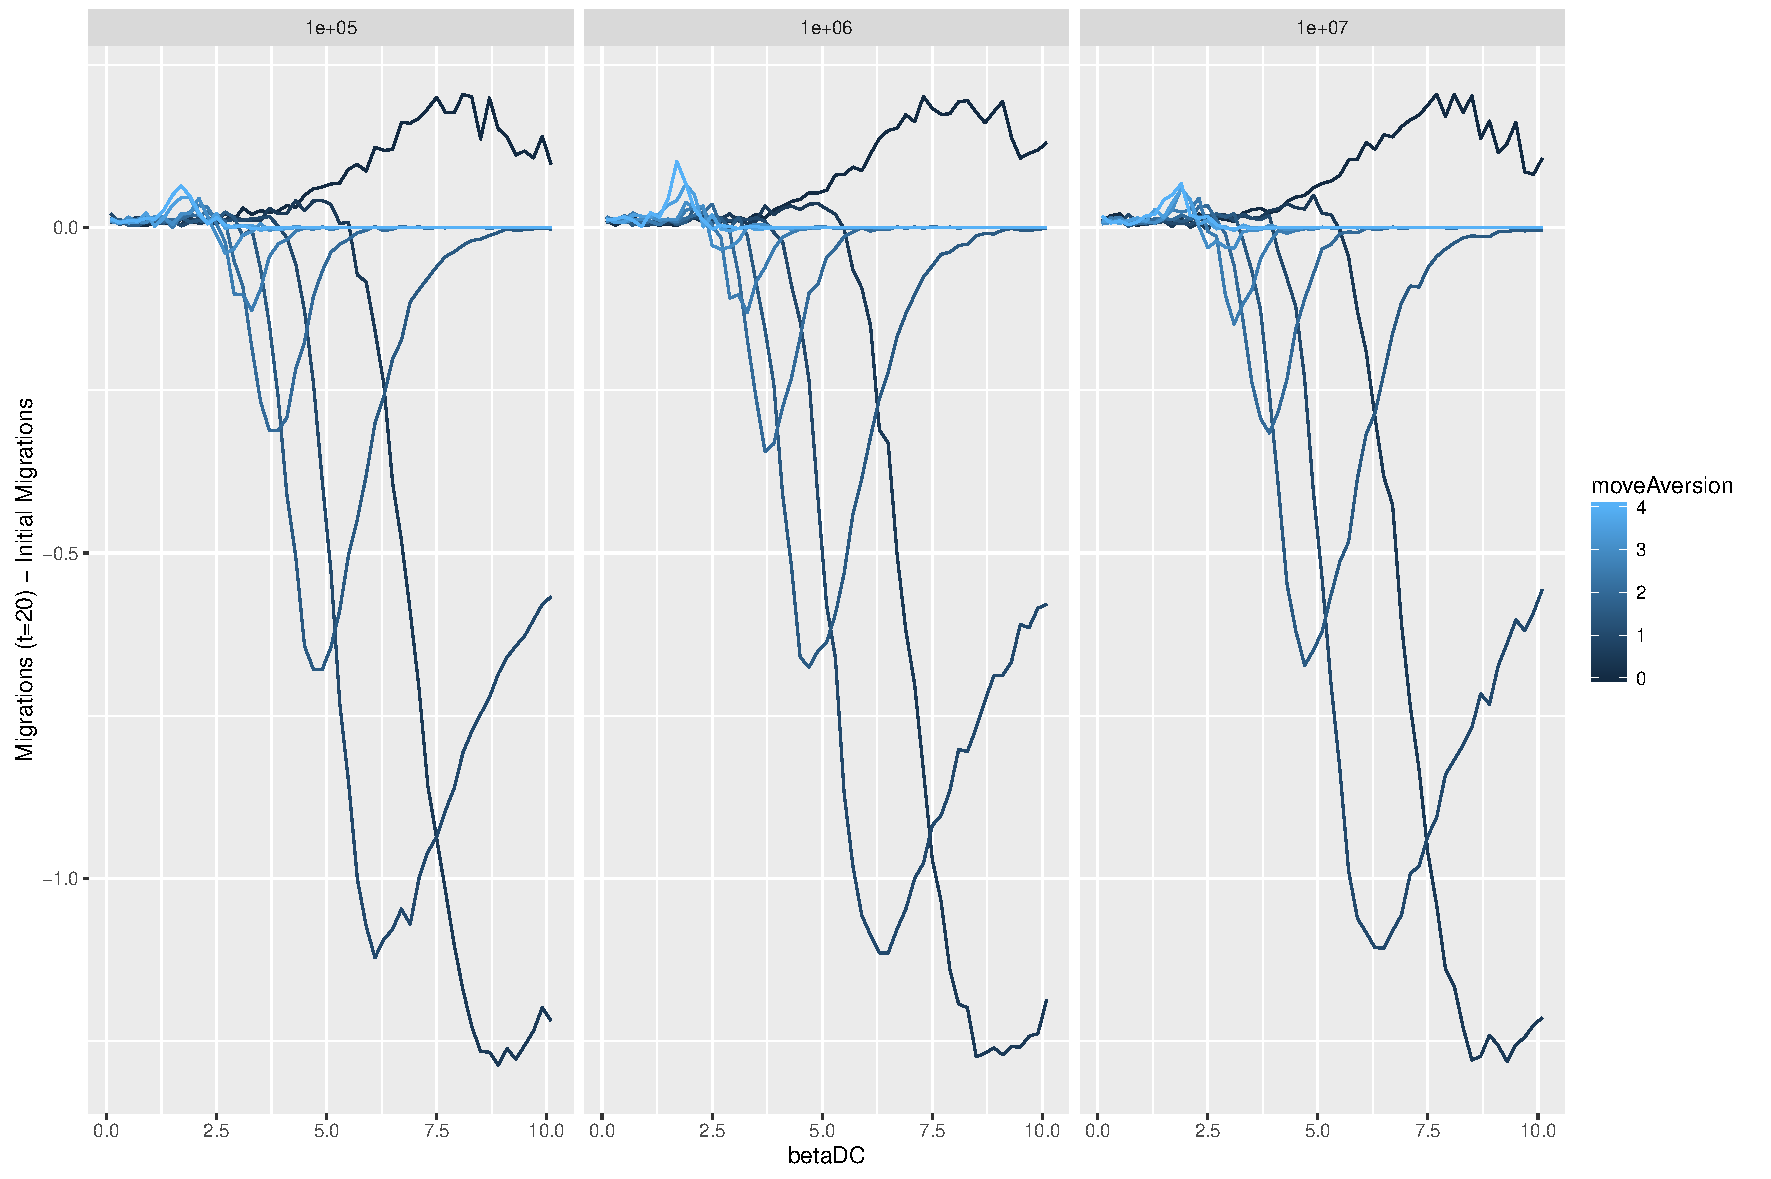
\includegraphics[width=\textwidth,height=0.3\textheight]{figures/migr-diff-final}
\caption{Difference in number of migrations between initial and final state of the model (relatively robust to final time).}
\label{fig:migr-diff}
\end{figure}
%%%%%%%%%%%%%%%%



%%%%%%%%%%%%%%%%%%%%
\subsection{Stylized Facts}

\paragraph{Role of economic categories}

\begin{itemize}
\item \textit{Adding categorisation does not change the qualitative behavior of the model. The lower category seems more vulnerable to spatial inequalities created by social determinism.}
\end{itemize}

\paragraph{Role of income growth}


\paragraph{Role of accessibility decay}





\paragraph{Sensitivity to Urban Form}

\comment[JR]{This sensitivity to meta-parameters may be an auxiliary question, but potentially interesting for planning/decision makers.}




%%%%%%%%%%%%%%%%%%%%
\subsection{Application : Real Configuration}



\paragraph{Stylized Pearl River Delta configuration}

The model is parametrized on a simplified configuration, with the sufficient information at the relevant scale: even if population data for example can be used with a very high resolution, it makes no sense regarding model ontology to include too precise GIS data as the city growth mechanisms are approximated processes. An correspondence between population and employment data is furthermore desirable, the former being available only at the scale of cities.


\paragraph{Comparing regulation policies}

Governments at different levels (national directives, regional policies, and municipal implementation \comment[JR]{check that}) try to regulate migration patterns. A point-based mechanism, a sort of ``social score'', has been tested for regulating urban Hukou. We stylize such policies by emphasizing their spatial aspect : across municipalities, there exist different incentives or dissuasions to migrate for some categories of migrants.


\paragraph{Experience Plan}

Concrete qualitative questions that can be asked to the model are for example:

\begin{itemize}
\item what is the impact of varying wealth distribution shape and width on system dynamics/migrant trajectories ?
\item what is the impact of various spatial distribution of $h_j^{(c)}$, i.e. different government policies ? We stylize existing policies that qualitative studies have unveiled.
\item Comparison with and without Hong-Kong and Macao \comment[JR]{I'm not sure this point is a good idea, as interactions processes are quite different (e.g. daily commuting, different migration rules, etc.) and it would become a gaz factory to include them in the model, like coupling three different models : one for mainland China, one for HK and Macao, and one for the cross-border flows.}
\end{itemize}




%%%%%%%%%%%%%%%%%%%%
\subsection{Summary of Stylized facts}

From the baseline behavior we learn that :

\begin{itemize}
\item When migrants have a high propensity to move, the spatial repartition of jobs becomes suboptimal in intermediate regimes of stochasticity, corresponding to a regime where congestion dominates. More precisely, we use a ``Random Utility'' specification for migrants' decisions, that includes a parameter $\beta$ that represents a ``level of randomness'' (or stochasticity) : when it goes to 0, migrations are totally random and without any sense, when it goes to infinity, migrants follow deterministically the best choice between staying and going to the best migration patch (depending on the sign of $\Delta U$). For intermediate values of $\beta$, we observe this congestion phenomenon.
\item The congestion regime corresponds to a linear decrease of job distance with randomness, meaning that social determinism creates spatial inequalities. It means that proximity to job is correlated with more congestion, but there is no direct causality between the two, both are outcome of model processes.
\item Changing the relative importance of accessibility does not affect much the aggregated dynamics: an increased gain in mobility produced by policies such as individual transportation subsidies will have no effect on migrations patterns. Accessibility is a generic notion to capture patterns of accessibility to urban functions and amenities ; in our case we use generalized Hansen accessibility, which can be understood in a simplified way number of jobs available to the population within a spatial range.
\item Configurations with an intermediate value of move aversion \comment{(CL) What does that mean?}[It corresponds to parameters in which people are not totally fixed neither totally mobile] (in which real configurations fall) yield a negative feedback effect to time, witnessing a progressive saturation. In a ``U-shape'' manner, very mobile or very fixed configurations yield positive feedback of time.
\end{itemize}

Comparing baseline configurations with one and two economic categories :

\begin{itemize}
\item Adding categorisation does not change the qualitative behavior of the model. It does not mean that categorization (based on professional qualifications, education, and economic situation) does not influence the migration behavior. In practice for example the points-based hukou system favoring “talents” – people with more qualifications, with stable job and economic situation etc. – can have a significant influence on migration behavior. It changes the migration behavior for individuals, but not the global qualitative picture of the previous stylized facts. %I have to think more on this and I totally agree on your second point : an interesting thing to try when testing the Hukou policies in the model is to check if we have the same phenomenon, and then to compare the effectiveness of policies at the individual level (impact on migrants trajectories) to the global level (behavior of the model).
The lower category seems more vulnerable to spatial inequalities created by social determinism.
\end{itemize}

Concerning the influence of economic parameters, namely income inequality and income growth, we find that :

\begin{itemize}
\item 
\end{itemize}

The introduction of real world data slightly changes conclusions :

\begin{itemize}
\item 
\end{itemize}

Finally, we compare stylized policies :

\begin{itemize}
\item 
\end{itemize}





%%%%%%%%%%%%%%%%%%%%
%% Biblio
%%%%%%%%%%%%%%%%%%%%

\bibliographystyle{apalike}
\bibliography{biblio}


\end{document}
